% Created 2011-05-23 Mon 11:39
\documentclass[11pt,english]{article}
\usepackage[utf8]{inputenc}
\usepackage[T1]{fontenc}
\usepackage{fixltx2e}
\usepackage{graphicx}
\usepackage{longtable}
\usepackage{float}
\usepackage{wrapfig}
\usepackage{soul}
\usepackage{textcomp}
\usepackage{marvosym}
\usepackage{wasysym}
\usepackage{latexsym}
\usepackage{amssymb}
\usepackage{hyperref}
\tolerance=1000

\usepackage{lmodern}
\renewcommand{\sfdefault}{lmss}
\renewcommand{\ttdefault}{lmtt}

% needed packages
\usepackage{amsmath}
\usepackage{amssymb}
\usepackage{amsthm}
\usepackage{babel}
\usepackage{epsfig}
\usepackage[T1]{fontenc}
\usepackage{fixltx2e}
\usepackage{float}
%\usepackage{floatflt}
\usepackage{graphics}
\usepackage{graphicx}
\usepackage[utf8]{inputenc}
\usepackage{latexsym}
\usepackage{longtable}
\usepackage{makeidx}
\usepackage{marvosym}
\usepackage{multicol}
%\usepackage{pslatex}
\usepackage{rotating}
%\usepackage{showidx}
\usepackage{soul}
\usepackage{srcltx}
\usepackage{stmaryrd}
\usepackage{subfig}
\usepackage{textcomp}
%\usepackage{theorem}
%\usepackage[subfigure]{tocloft}
\usepackage{txfonts}
\usepackage{upgreek}
\usepackage{url}
\usepackage{varioref}
%\usepackage{wasysym}
\usepackage{wrapfig}


% Page setup
\usepackage[paperwidth=8.5in,paperheight=11in]{geometry}
\geometry{verbose,tmargin=0.5in,bmargin=0.5in,lmargin=1in,rmargin=1in}




% PDF settings
%\usepackage[hyperref,x11names]{xcolor}
\usepackage{hyperref}
\hypersetup{pdftitle={STAT 5840: Statistical Computing},
 		pdfauthor={G. Jay Kerns}, 
		linkcolor=Firebrick4, 
		citecolor=black, 
		urlcolor=SteelBlue4}

% Listings setup
%\usepackage{color}
%\usepackage{listings}
%\lstset{basicstyle={\ttfamily},
%	language=R,
%	breaklines=true,
%	breakatwhitespace=true,
%	keywordstyle={\ttfamily},
%	numberstyle = {\ttfamily},
%	morestring=[b]"
%}



%  user defined commands
% special operators
\renewcommand{\P}{\mathrm{I\hspace{-1.5pt}P}}
\newcommand{\E}{\mathrm{I\hspace{-1.5pt}E}}
\renewcommand{\vec}[1]{\mbox{\boldmath$#1$}}

% special symbols
\newcommand{\me}{\mathrm{e}}
\newcommand{\R}{\mathbb{R}}
\newcommand{\diff}{\mathrm{d}}
\newcommand{\ybar}{\overline{y}}
\newcommand{\xbar}{\overline{x}}
\newcommand{\Xbar}{\overline{X}}
\newcommand{\Ybar}{\overline{Y}}





\providecommand{\alert}[1]{\textbf{#1}}

\title{Illustration of the Accept/Reject Algorithm}
%\author{G. Jay Kerns}
\date{STAT 5840: Summer 2011}

\begin{document}

\maketitle

\thispagestyle{empty}

\section*{Discrete Accept/Reject}
\label{sec-1}

This function generates a discrete distribution via the accept-reject algorithm.  Copy-paste the \texttt{mydiscretev} function at the command prompt in \texttt{R}.
\begin{verbatim}
# mydiscretev.R

mydiscretev <- function(p,N){
  # mydiscretev.R
  # p is the desired target density on 1,...,k.
  # N is the number of observations desired
  x <- rep(0, times = N)                # initialize
  k <- length(p)                        # the support of p
  M <- k*max(p)                         # the bound size
  for(i in seq.int(N)){
    accept <- FALSE                     # initialize
    while (!accept){                    # continue until we accept
      y <- sample(k, size = 1)          # y is disc unif 1...k
      u <- runif(1)                     # u is unif(0,1)
      accept <- ( u < p[y]/(M*1/k) )    # is TRUE if A/R condition satisfied
    }
    x[i] <- y                           # this y is a good one
  }
  return(x)
}
\end{verbatim}
After copy-pasting we can run the function with the following.
\begin{verbatim}
p <- c(.11, .12, .09, .08, .12, .10, .09, .09, .10, .10)
x <- mydiscretev(p, 10000)
\end{verbatim}


\begin{verbatim}
plot(prop.table(table(x)), ylab = "Relative frequency")
\end{verbatim}

\begin{figure}[h!]
\centering
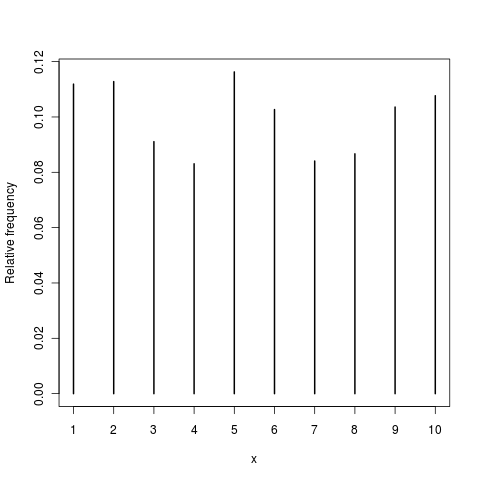
\includegraphics[width=6in, height=6in,]{img/DARalgo.pdf}
\caption{\label{fig:yplot}A relative frequency barplot of the simulated values}
\end{figure}

\end{document}